\section{Esempio di funzionamento}

In questo esempio di funzionamento si utilizzerà il gene ENSG00000280145, situato nel cromosoma 21 dell'uomo sapiens (GRCh38 / hg38). E' stato prima scaricato il   genoma di riferimento da ensembl in formato fasta e la relativa annotazione in formato gtf. Dal file gtf (contenente l'annotazione per l'intero genoma) è stata isolata l'annotazione relativa al gene ENSG00000280145.

\subsection{Generazione delle read}

Si è scelto di utilizzare Flux Simulator per la generazione delle read paired-end. Il suo utilizzo non è particolarmente complicato, ma è necessario passare i diversi parametri attraverso un file con estensione .p. Il file utilizzato in questa simulazione è il seguente:

\begin{figure}[h]
	\centering
	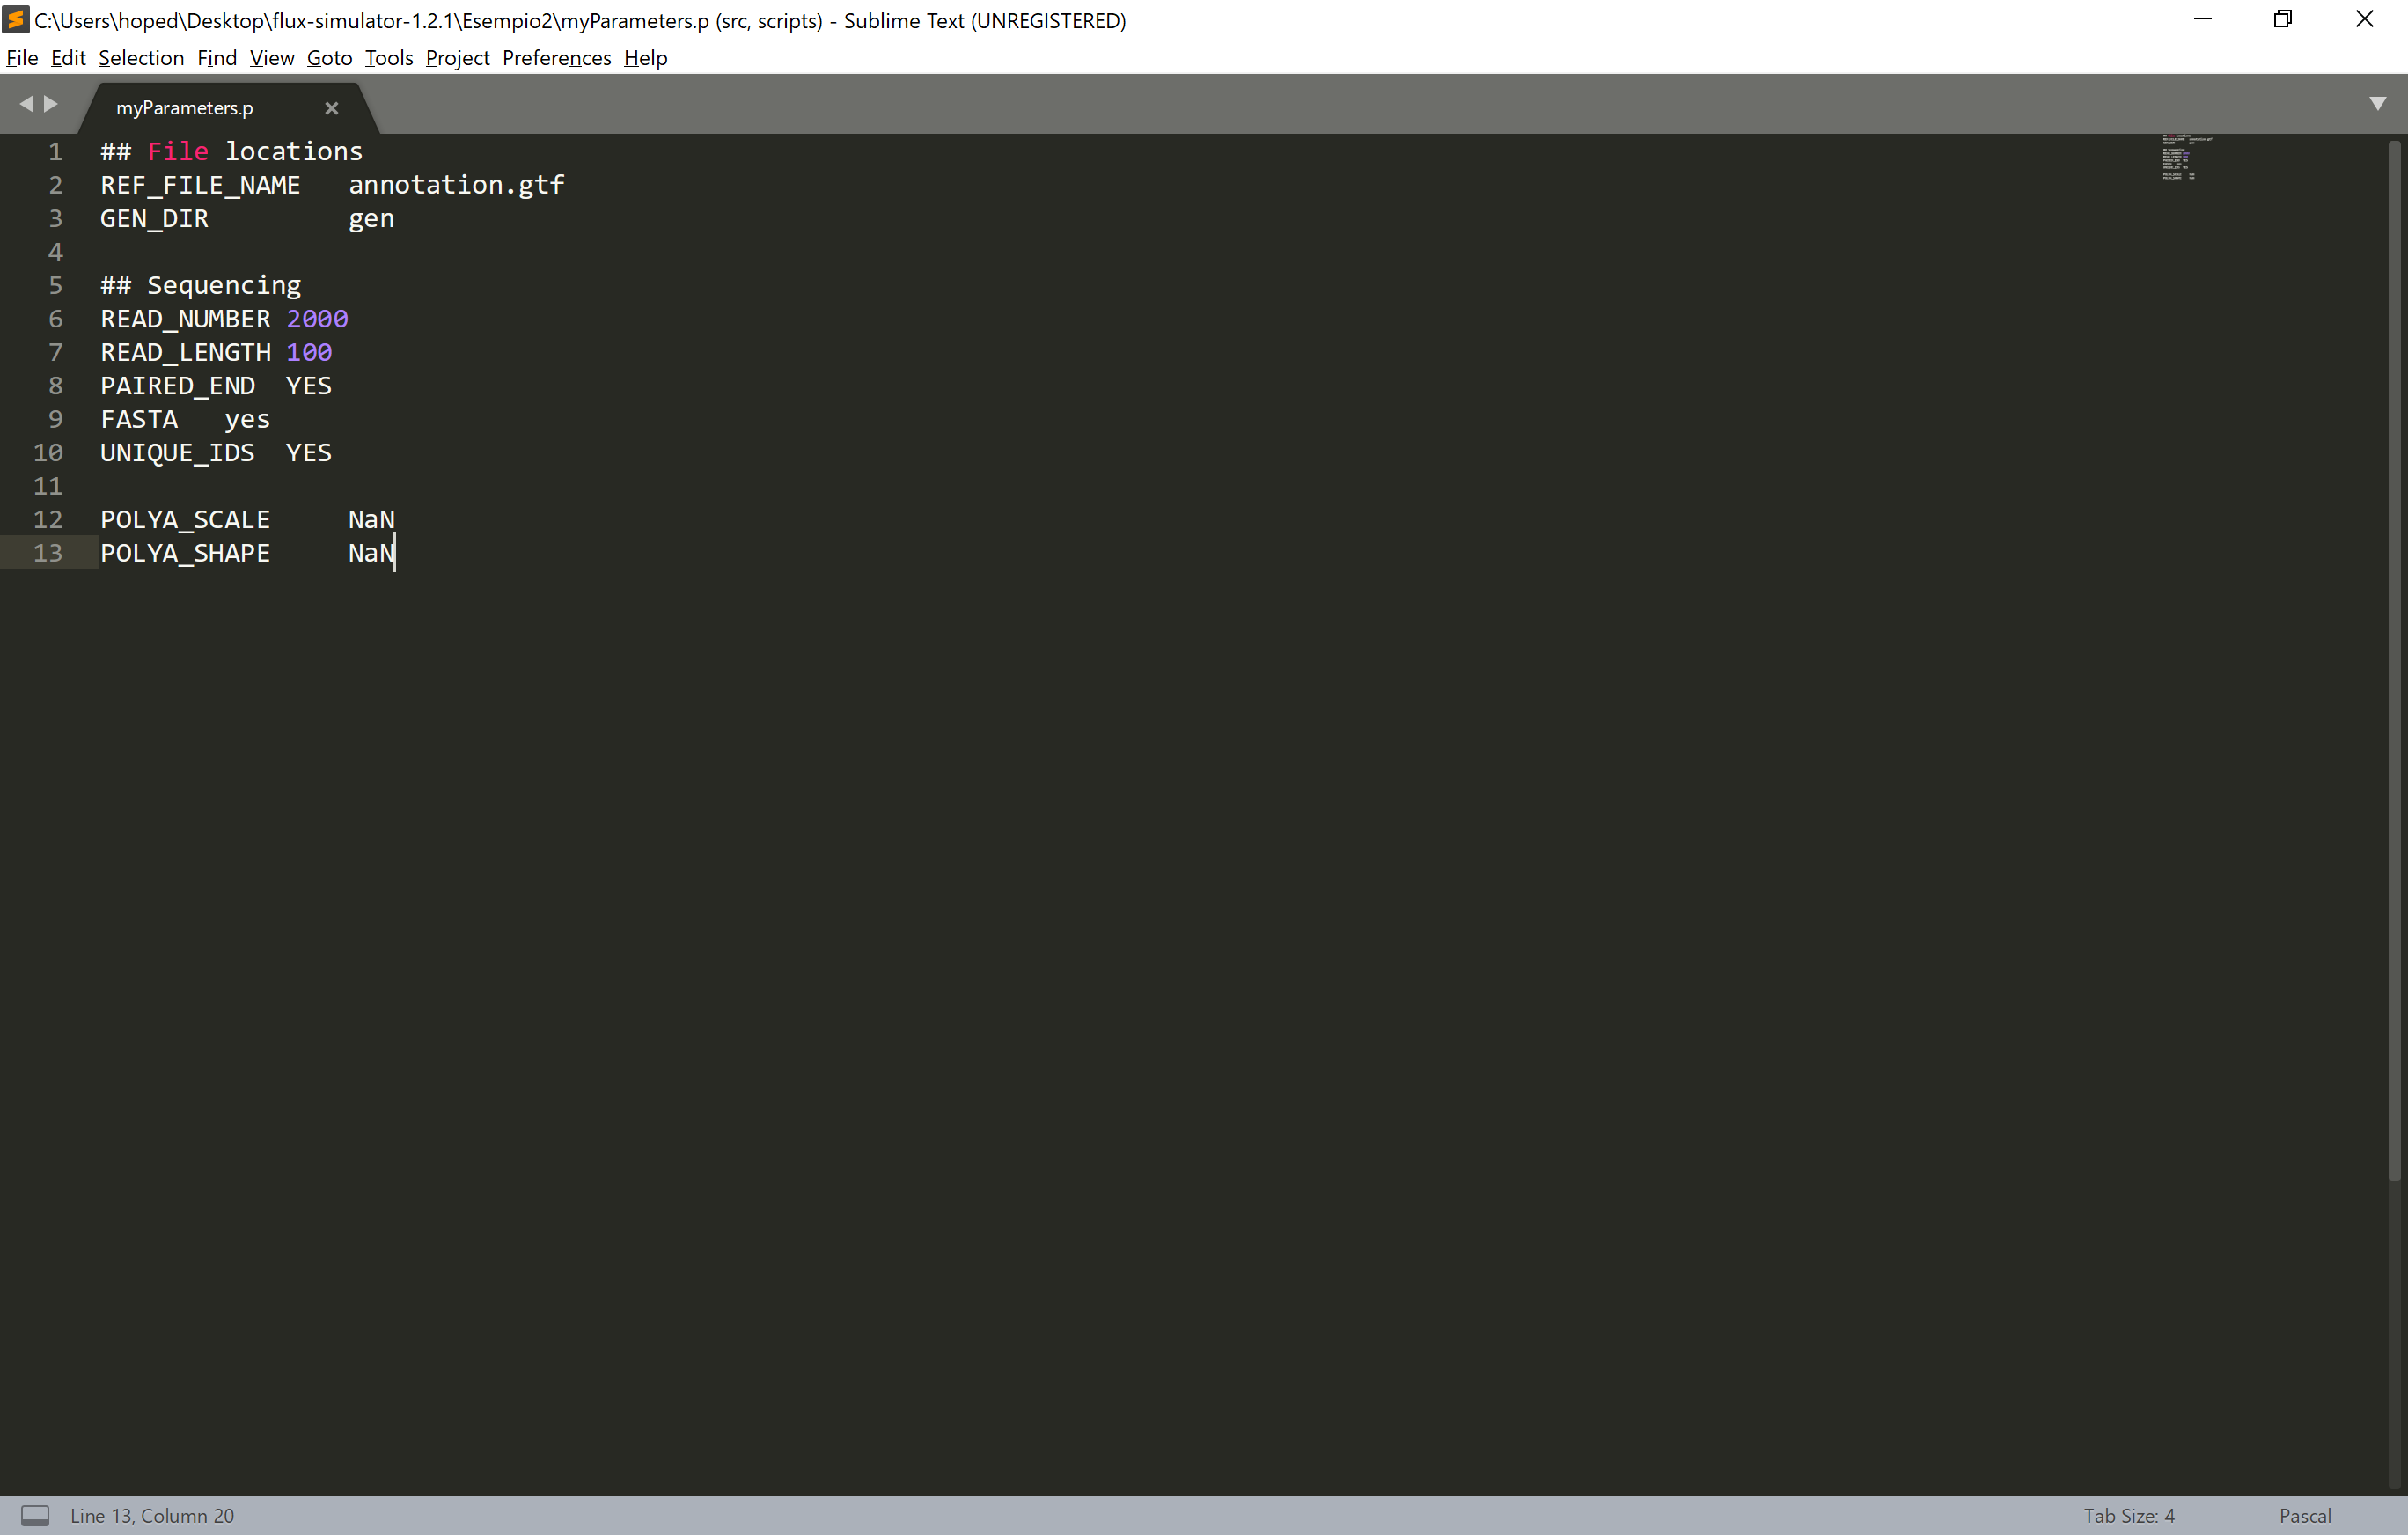
\includegraphics[width=\linewidth]{images/parameters.png}
  \caption{Il file contente i parametri di Flux Simulator}
  \label{fig:Parameters}
\end{figure}

Vengono così generati due file contenti 2000 read di lunghezza 100, in formato fasta, che saranno dati in input ad ASGAL.

\newpage

\subsection{Utilizzo}

ASGAL viene eseguito via linea di comando, richiamando lo script principale usando come parametri:

\begin{itemize}
	\item Il genoma di riferimento (opzione -g)
	\item L'annotazione del genoma (opzione -a)
	\item I due file contenti read (opzioni -s e -s2)
	\item La cartella di destinazione dell'output (opzione -o)
	\item L'indicazione delle read paired-end (opzione --paired)
	\item La fragment library type (opzione -f), opzionale per velocizzare la fase di allineamento
\end{itemize}

Questo script richiama nell'ordine lo Splice-Aware Aligner, il Formattatore SAM e il Rilevatore di eventi di Alternative Splicing, visualizzando alcune informazioni sul funzionamento.

Questa immagine mostra il funzionamento di ASGAL:

Sebbene sia possibile eseguire ciascuno script singolarmente, si raccomanda di usare lo script principale per un utilizzo più immediato. 

\newpage

\subsection{Risultati}

Sono stati rilevati i seguenti eventi di Alternative Splicing:



\newpage